En esta sección, se presentan los resultados obtenidos al reproducir cada uno de
los experimentos de la sección anterior, es decir, los experimentos que los autores
presentan en su trabajo \cite{jsantos-amonteagudo-1-2014}.

Antes de todo, hay que tener en cuenta la componente aleatoria de la simulación. Esto es, por
la realización de sorteos de cara a ejecutar la mitosis u otra acción. En consecuencia, la aparición
de un marcador u otro, como se verá a continuación, provoca alteraciones en la simulación, de modo que
el comportamiento puede variar. En este caso, lo que se pretende es llegar a la misma conclusión que los autores,
por tanto, el análisis de los resultados propios debe hacerse con ese objetivo en mente.

\section{Influencia del parámetro \textit{Tasa de mutación base (m)}}

Las células de la simulación, y como se ha descrito en secciones previas, tienen asociado una propiedad que está relacionada con la aparición
de nuevas mutaciones durante la mitosis, este es, el parámetro \textit{tasa de mutación base} o $m$. En este experimento,
se pretende someter a la simulación a diferentes configuraciones de este parametros para estudiar qué
progresión presentan los tumores.

Se parte de una probabilidad de aparición de mutaciones baja, ya que, el sorteo se efectúa con una probabilidad de
$1/m$, por lo que, a mayor valor del parámetro $m$, menor probabilidad de que ocurra. En este caso, se
realizan tres simulaciones, para $m=10.000$, $m=1.000$ y $m=100$.

\subsection{Experimento 1: Tasa de mutación base igual a 10.000}

En la primera de las tres figuras, la figura~\ref{fig:ownexp1-1}, se presenta el resultado
de la simulación desde el punto de vista de las células sanas y las células cancerosas.

\begin{figure}[h]
\centering
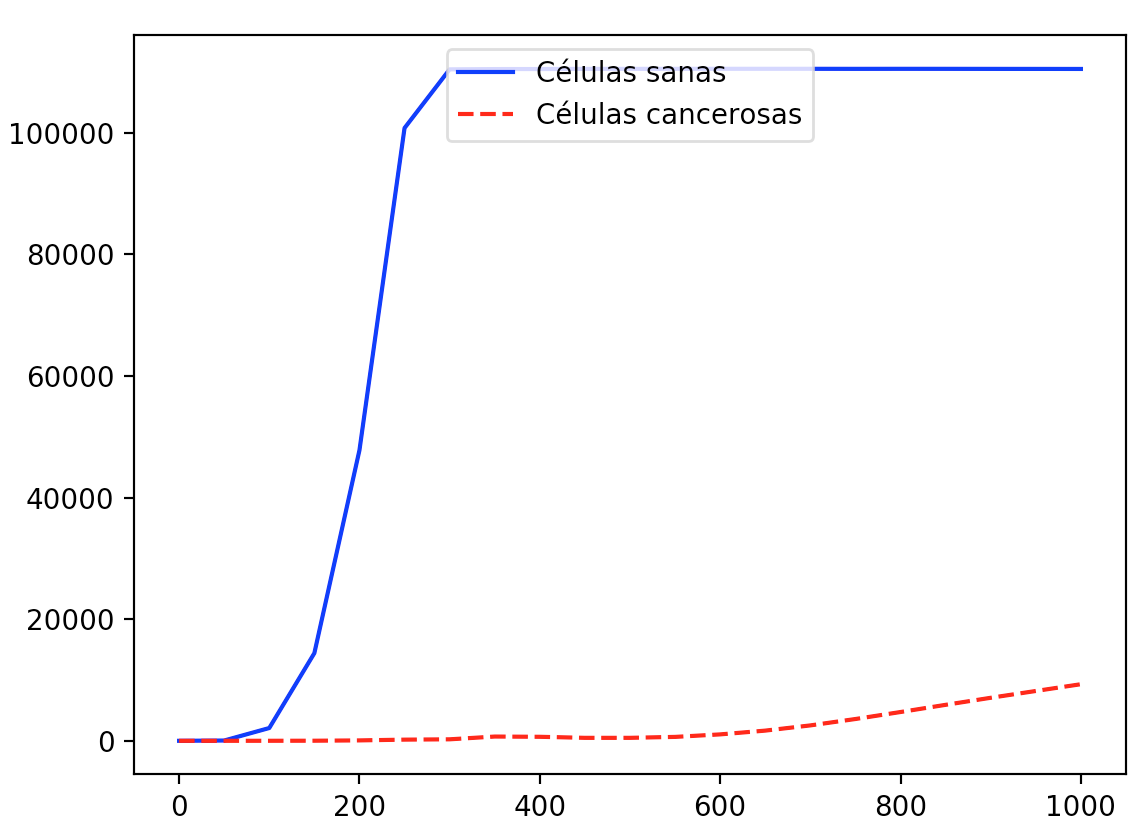
\includegraphics[scale=0.6]{figures/experiments/exp1/healthvscarcino}
\caption{Células sanas frente a células cancerosas como resultado de la simulación para el experimento con $m = 10.000$.}
\label{fig:ownexp1-1}
\end{figure}

El resultado obtenido es bastante similar, por lo que se debe observar la evolución de los
marcadores, la cual se presenta en la figura~\ref{fig:ownexp1-2}. En este caso, el marcador
más relevante es $SG$. Aunque, en este caso, se ha asociado a la mutación $EI$, el comportamiento
global se debe al marcador $SG$. Es decir, el tumor crece por la parte exterior de la rejilla que,
como se ha descrito en el capítulo anterior, se debe a un menor factor de crecimiento. El marcador
$EI$ surge en una de esas células y evoluciona sin alterar el comportamiento global.

\begin{figure}[h]
\centering
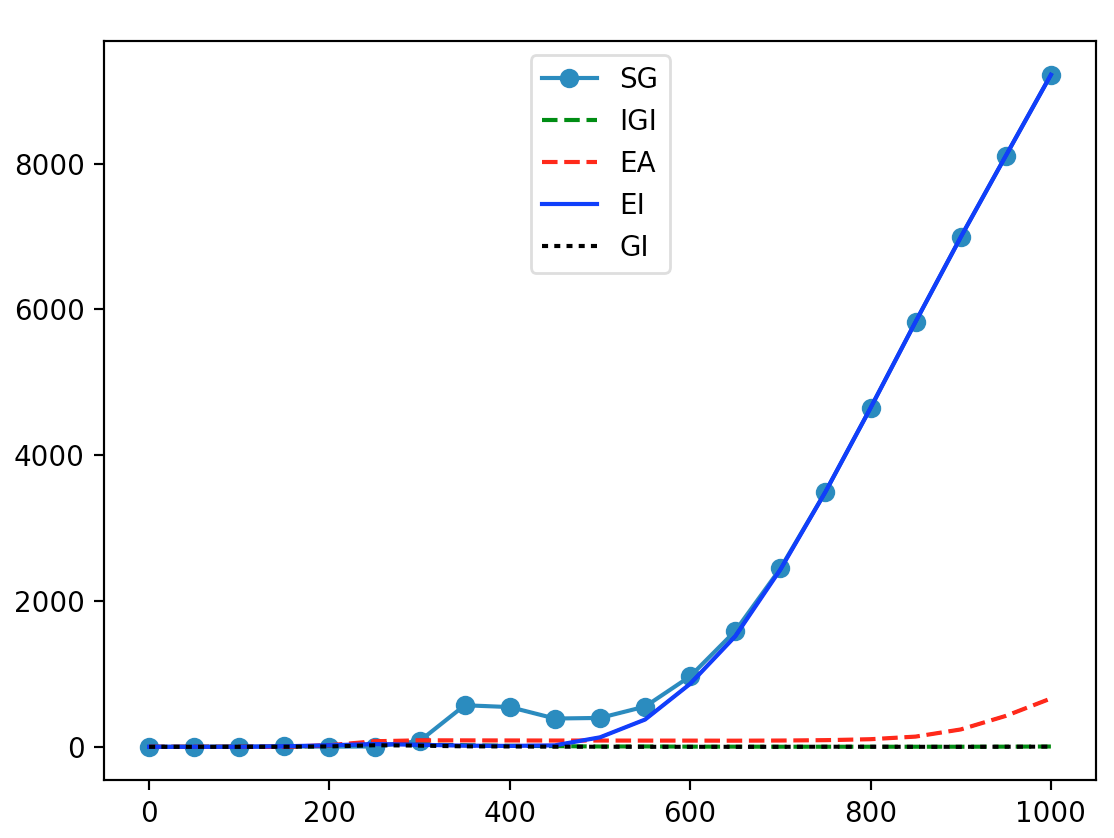
\includegraphics[scale=0.6]{figures/experiments/exp1/mutations}
\caption{Evolución de los marcadores como resultado de la simulación para el experimento con $m = 10.000$.}
\label{fig:ownexp1-2}
\end{figure}

En una vista de la rejilla, como en la~\ref{fig:ownexp1-3}, se puede observar como
efectivamente tiende a ocupar el exterior, lo que coincide con los resultados obtenidos por los
autores.

\begin{figure}[h]
\centering
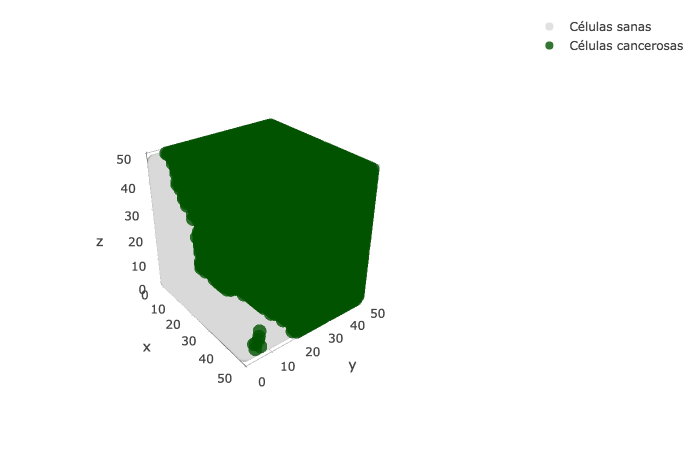
\includegraphics[scale=0.6]{figures/experiments/exp1/grid}
\caption{Rejilla resultante de la simulación para el experimento con $m = 10.000$.}
\label{fig:ownexp1-3}
\end{figure}

\clearpage

\subsection{Experimento 2: Tasa de mutación base igual a 1.000}

En la primera de las tres figuras, la figura~\ref{fig:ownexp2-1}, se presenta el resultado
de la simulación desde el punto de vista de las células sanas y las células cancerosas,
pero en esta ocasión con el parámetro establecido a $m=1.000$.

\begin{figure}[h]
\centering
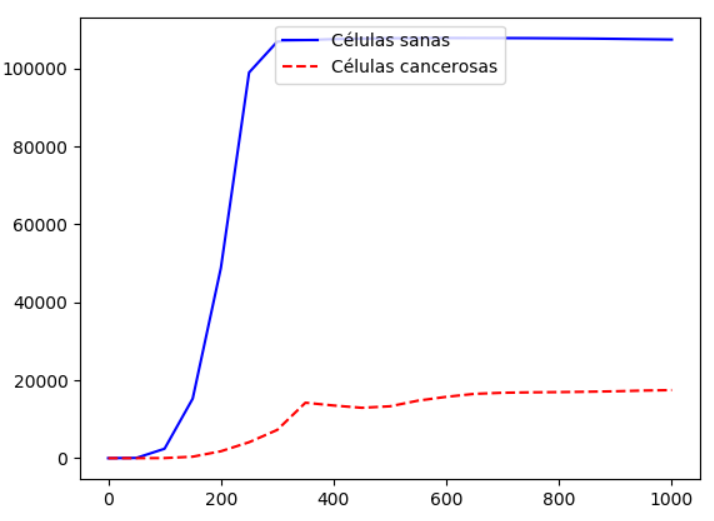
\includegraphics[scale=0.8]{figures/experiments/exp2/healthvscarcino}
\caption{Células sanas frente a células cancerosas como resultado de la simulación para el experimento con $m = 1.000$.}
\label{fig:ownexp2-1}
\end{figure}

El resultado obtenido es bastante similar, por lo que se debe observar la evolución de los
marcadores, la cual se presenta en la figura~\ref{fig:ownexp2-2}. En este caso, el marcador
más relevante es $SG$. Aunque, en este caso, se ha asociado también a la mutación $EI$. El segundo marcador
más relevante tras $SG$, es el marcador $EA$. Este comportamiento se observa también en
los resultados obtenidos por los autores.

\begin{figure}[h]
\centering
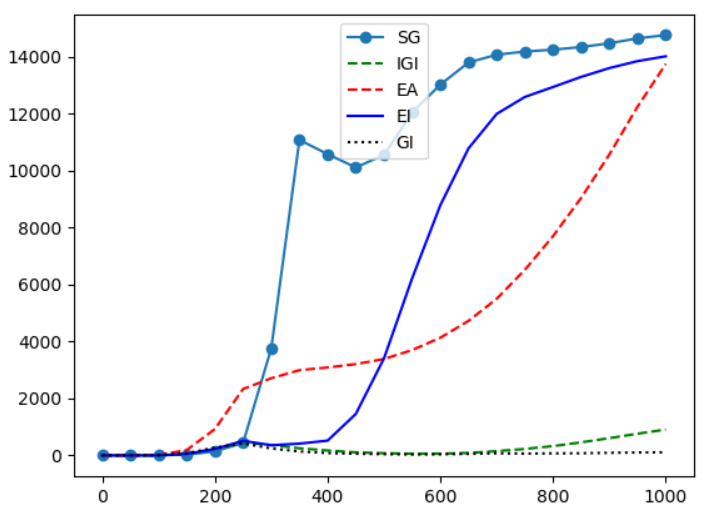
\includegraphics[scale=0.8]{figures/experiments/exp2/mutations}
\caption{Evolución de los marcadores como resultado de la simulación para el experimento con $m = 1.000$.}
\label{fig:ownexp2-2}
\end{figure}

En una vista de la rejilla, como en la~\ref{fig:ownexp2-3}, se puede observar como
tiende a ocupar el exterior y, en este caso, también una pequeña parte del espacion
interior de la rejilla, lo que coincide con los resultados obtenidos por los
autores.

\begin{figure}[h]
\centering
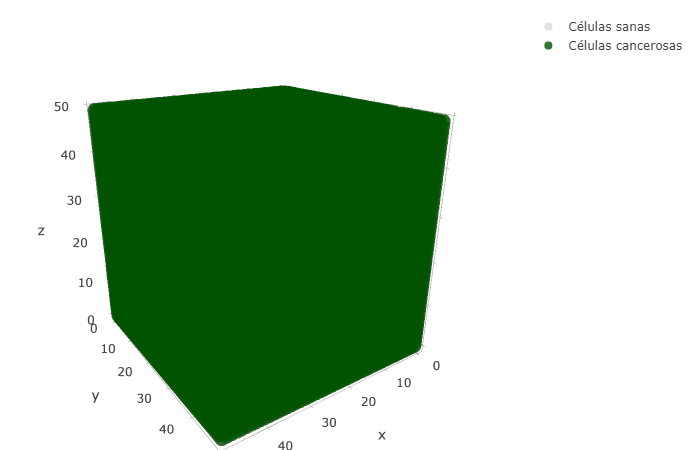
\includegraphics[scale=0.6]{figures/experiments/exp2/grid}
\caption{Rejilla resultante de la simulación para el experimento con $m = 10.000$.}
\label{fig:ownexp2-3}
\end{figure}

\clearpage

\subsection{Experimento 3: Tasa de mutación base igual a 100}

En la primera de las tres figuras, la figura~\ref{fig:ownexp3-1}, se presenta el resultado
de la simulación desde el punto de vista de las células sanas y las células cancerosas,
pero en esta ocasión con el parámetro establecido a $m=100$.

\begin{figure}[h]
\centering
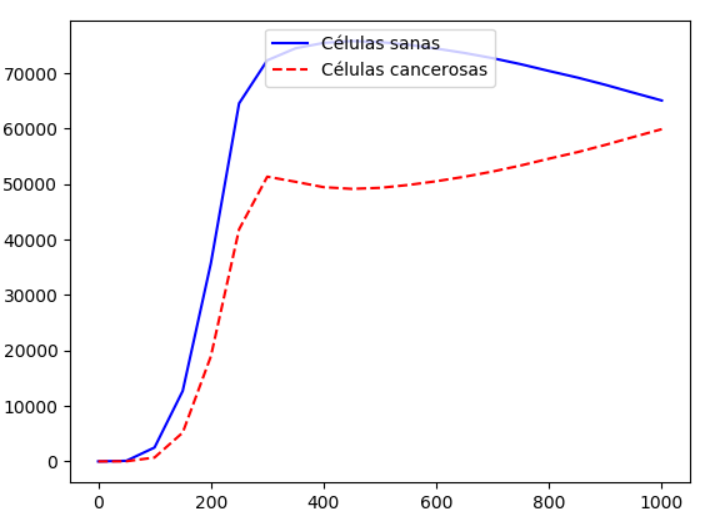
\includegraphics[scale=0.8]{figures/experiments/exp3/healthvscarcino}
\caption{Células sanas frente a células cancerosas como resultado de la simulación para el experimento con $m = 100$.}
\label{fig:ownexp3-1}
\end{figure}

El resultado obtenido aquí es difernte a priori. El número de células cancerosas
no supera rápidamente al de células sanas, por el contrario, al final de la simulación
se observa como si hubiera más iteraciones pronto llegarían a representar la inmensa
totalidad de la rejilla.

Esto se explica por la evolución de los marcadores de dicha simulación, como se muestra en
la figura~\ref{fig:ownexp3-2}. El marcador $EA$ presenta un comportamiento similar, pero
no es suficiente por sí solo. En este caso, la menor presencia del marcador $IGI$, el cual
permite superar el límite de la falta de espacio que tiene lugar en la zona interior de la rejilla,
provoca que no superen en número las células cancerosas a las sanas.

\begin{figure}[h]
\centering
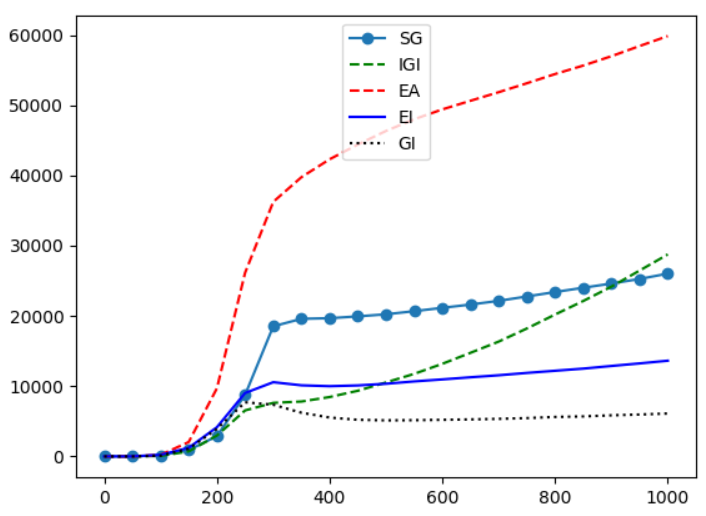
\includegraphics[scale=0.8]{figures/experiments/exp3/mutations}
\caption{Evolución de los marcadores como resultado de la simulación para el experimento con $m = 100$.}
\label{fig:ownexp3-2}
\end{figure}

Aunque, desde el punto de vista de la rejilla, como se muestra en la figura~\ref{fig:ownexp3-2},
el comportamiento es parecido salvando los detalles comentados anteriormente. Es decir,
hay mayor presencia de células cancerosas en la zona interior.

\begin{figure}[h]
\centering
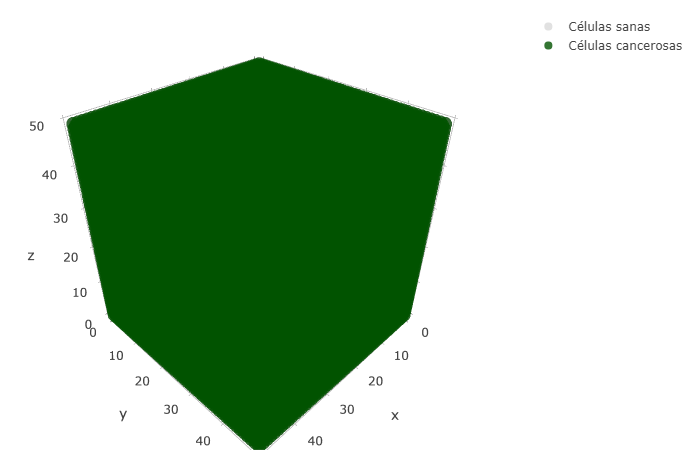
\includegraphics[scale=0.6]{figures/experiments/exp3/grid}
\caption{Rejilla resultante de la simulación para el experimento con $m = 100$.}
\label{fig:ownexp3-3}
\end{figure}

\clearpage

\section{Influencia del resto de parámetros}

Para comprobar la influencia del resto de parámetros que intervienen en la simulación,
los autores realizan una modificación de los mismos. En la tabla 6.2 se muestran los valores
utilizados en esta ocasión, alterando el tamaño del telómero ($tl$), lo que supone
menos oportunidades de división de la célula original y de sus descendientes, entre otros
cambios.

\begin{table}[h!]
  \centering
  \caption{Valores de los parámetros.}
  \label{tab:table1}
  \begin{tabular}{ccc}
    \toprule
    Nombre & Símbolo & Valor\\
    \midrule
    Tasa de mutación base & m & 100.000\\
    Tamaño del telómero & tl & 35\\
    Muerte por daño genético & e & 20\\
    Factor de incremento de tasa de mutación base & i & 100\\
    Muerte de un vecino & g & 10\\
    Muerte aleatoria & a & 400\\
    \bottomrule
  \end{tabular}
\end{table}

Las pruebas anteriores sirven para comprobar la dificultad de aparición del cáncer en
función del parámetro $m$. La configuración inicial es la misma que en los experimentos
anteriores, exceptuando el número de iteraciones, que en este caso asciende a $5.000$.

Los resultados obtenidos se muestran a continuación.

\begin{figure}[h]
\centering
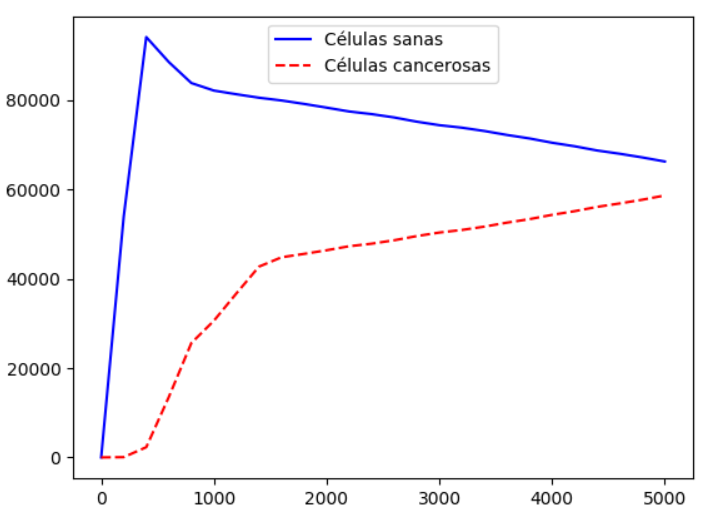
\includegraphics[scale=0.8]{figures/experiments/exp4/healthvscarcino}
\caption{Células sanas frente a células cancerosas como resultado de la simulación para el experimento con $m = 100.000$.}
\label{fig:ownexp4-1}
\end{figure}

Desde el punto de vista del número de células sanas frente a cancerosas, el resultado es
bastante similar, como se puede ver en la figura~\ref{fig:ownexp4-1}.

\begin{figure}[h]
\centering
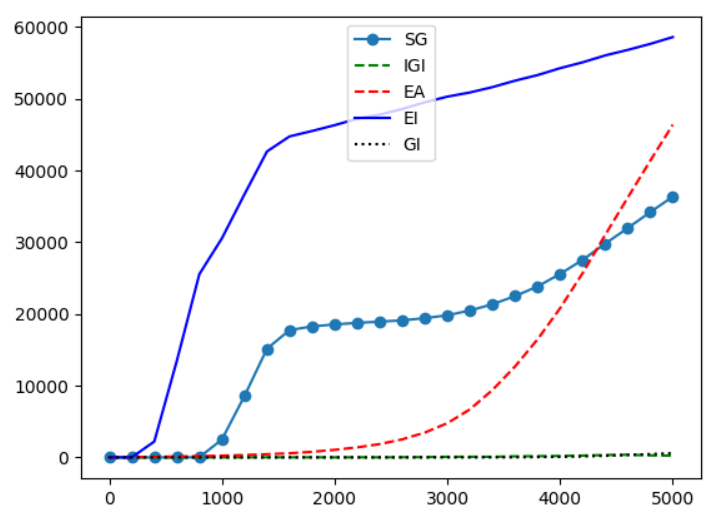
\includegraphics[scale=0.8]{figures/experiments/exp4/mutations}
\caption{Evolución de los marcadores como resultado de la simulación para el experimento con $m = 100.000$.}
\label{fig:ownexp4-2}
\end{figure}

Para observar esto con más detalle, en la figura~\ref{fig:ownexp4-2}, se observa el comportamiento
de los marcadores, resultando también bastante similar. El marcador más relevante es $EI$,
como ocurre en el experimento de los autores. Seguigo de $SG$ y $EA$ respectivamente. Un detalle
diferente, aunque irrelevante, es que el marcador $IGI$ no hace presencia al final de la
simulación como en el experimento de los autores. En este caso, en el experimento de los autores
su presencia es tan baja que apenas altera el resultado global.

Finalmente, el resultado de la rejilla para este experimento es similar al de la figura ~\ref{fig:ownexp3-3}.

\clearpage

\section{Influencia de parámetros con rejilla completa de células sanas}

En este caso, se parte con una rejilla completa de células sanas. En cuanto a los parámetros,
se utilizan los mismos que en la secciones anteriores. Primero una simulación de $8.000$ iteraciones
con los parámetros por defecto, y luego una segunda de $100.000$ iteraciones con los parámetros
utilizados en el experimento de la figura~\ref{fig:exp4}.

En este caso, la simulación se corresponde con una equivalencia temporal
de $2.3$ años y $29.7$ años respectivamente.

\begin{figure}[h]
\centering
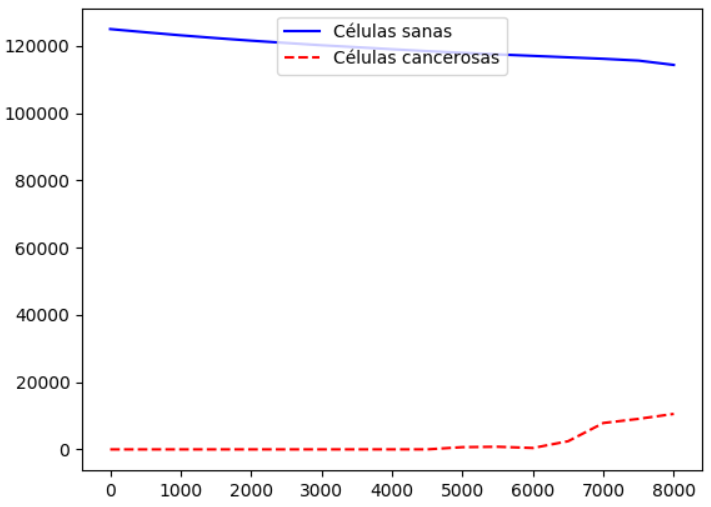
\includegraphics[scale=0.8]{figures/experiments/exp5/healthvscarcino}
\caption{Evolución de las células sanas frente a células cancerosas con rejilla completa de células sanas y parámetros por defecto.}
\label{fig:ownexp5-1}
\end{figure}

El resultado obtenido desde el punto de vista de las células sanas frente a células cancerosas
es similar. La única diferencia, como se observa en la figura~\ref{fig:ownexp5-1}, es
que el paso de las células cancerosas en número frente a las células sanas ocurre unas
$1.000$ iteraciones después que en el resultado obtenido por los autores.

\begin{figure}[h]
\centering
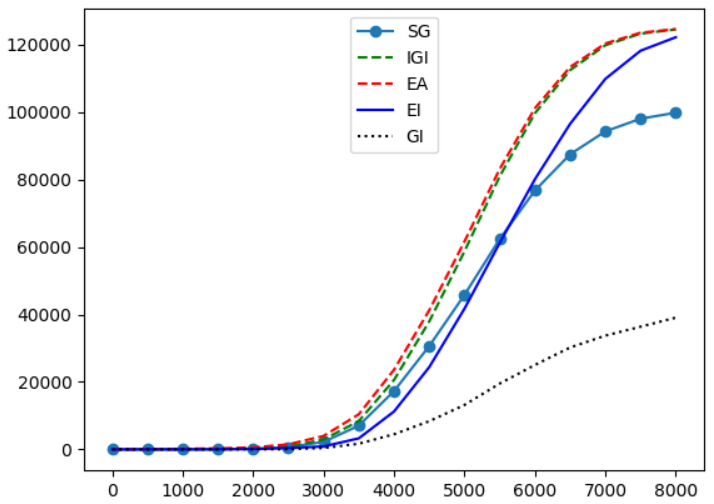
\includegraphics[scale=0.8]{figures/experiments/exp5/mutations}
\caption{Evolución de los marcadores cancerosos con rejilla completa de células sanas y parámetros por defecto.}
\label{fig:ownexp5-2}
\end{figure}

Desde el munto de vista de los marcadores, como se muestra en la figura~\ref{fig:ownexp5-2}, es muy
parecido. Como ambos comportamientos son similares a los obtenidos por los autores se entiende
que la explicación es la misma que se presenta en el capítulo anterior donde
se presentan los resultados de los autores.

Para finalizar este experimento, en la figura~\ref{fig:ownexp3-3} se muestra sobre la rejilla el resultado
obtenido al finalizar la simulación, que es similar al caso actual.

En otro experimento similar, pero alterando los parámetros de simulación como en el experimento de la sección
7.2, los resultados obtenidos se muestran a continuación.

\begin{figure}[h]
\centering
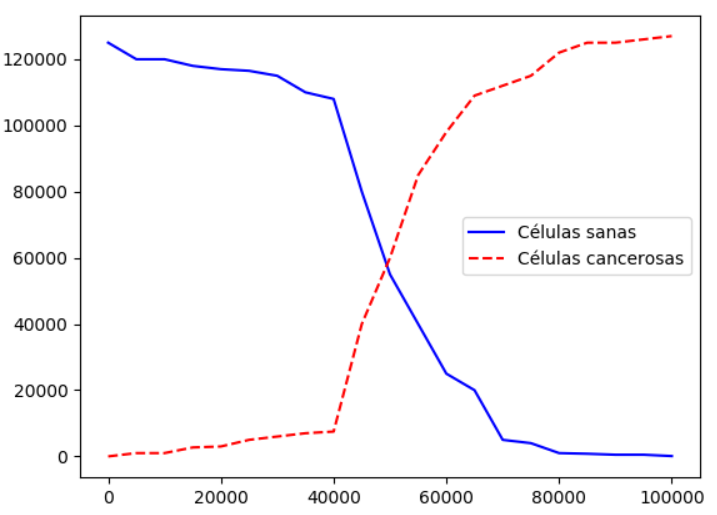
\includegraphics[scale=0.8]{figures/experiments/exp6/healthvscarcino}
\caption{Evolución de las células sanas frente a células cancerosas con rejilla completa de células sanas.}
\label{fig:ownexp6-1}
\end{figure}

El resultado obtenido desde el punto de vista de las células sanas frente a células cancerosas
es similar.

\begin{figure}[h]
\centering
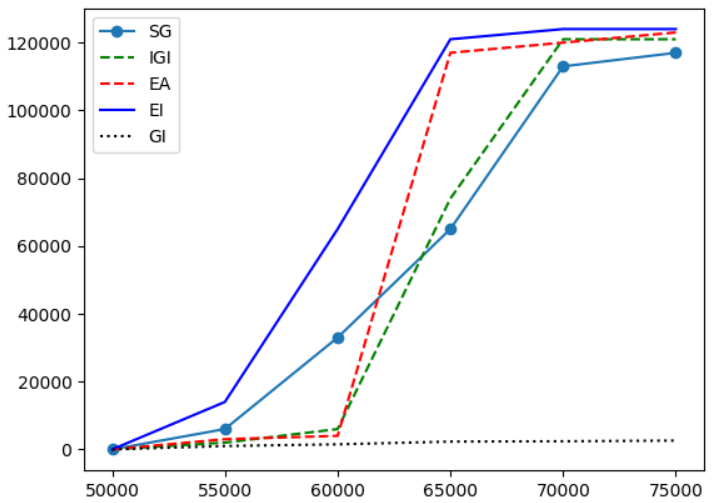
\includegraphics[scale=0.8]{figures/experiments/exp6/mutations}
\caption{Evolución de los marcadores cancerosos con rejilla completa de células sanas.}
\label{fig:ownexp6-2}
\end{figure}

Desde el munto de vista de los marcadores, como se muestra en la figura~\ref{fig:ownexp6-2}, es muy
parecido. Como ambos comportamientos son similares a los obtenidos por los autores se entiende
que la explicación es la misma que se presenta en el capítulo anterior donde
se presentan los resultados de los autores.

Para finalizar este experimento, en la figura~\ref{fig:ownexp3-3} se muestra un resultado sobre la rejilla similar que el
obtenido al finalizar esta simulación.

\clearpage

\section{Relevancia de los marcadores}

En este caso, se intenta responder a la siguiente pregunta: \textit{¿Cuál sería
el comportamiento emergente si algún marcador no estuviera presente y no aplicaran
sus efectos?}.

Conocer el efecto de cada marcador en el comportamiento emergente para crecimiento de tumores
puede resultar útil para mejorar las terapias contra el cáncer. Esto se debe a que una terapia
consiste en inhibir un determinado camino del cáncer, aunque diferentes drogas actúan contra marcadores específicos.

\begin{figure}[h]
\centering
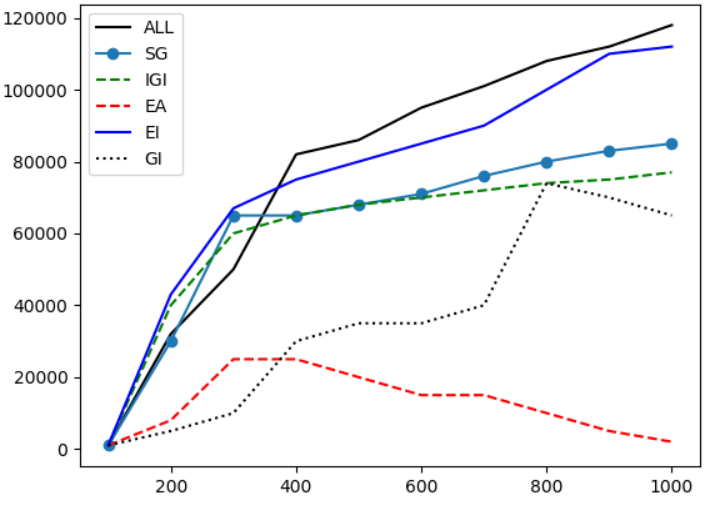
\includegraphics[scale=0.8]{figures/experiments/exp7/exp7-1}
\caption{Efecto de la eliminación de un marcador con parámetros por defecto excpeto con $m = 100$.}
\label{fig:ownexp7-1}
\end{figure}

\begin{figure}[h]
\centering
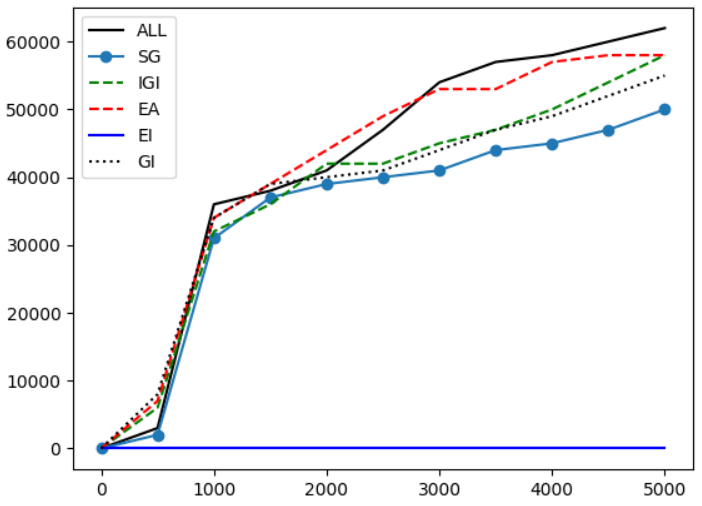
\includegraphics[scale=0.6]{figures/experiments/exp7/exp7-2}
\caption{Efecto de la eliminación de un marcador con parámetros del cuadro 7.1.}
\label{fig:ownexp7-2}
\end{figure}

En la figura~\ref{fig:ownexp7-1}, se observa el resultado de la simulación. En este caso, el marcador
más importante de acuerdo al crecimiento del tumor es $EA$,
porque su eliminación implica un alto decrecimiento en el número de células cancerosas.
Esto es, sin considerar $EA$, todos las células cancerosas tienen una probabilidad de morir
por apoptosis, así la proliferación del cáncer disminuye. Del análisis mostrado se extrae
que los siguientes marcadores más relevantes en este caso son $GI$ e $IGI$. La relevancia de $GI$
se explica porque cuando la rejilla está completa hay menor adquisición de mutaciones durante la división.
La relevancia de $IGI$ es explicada porque cuando la rejilla está completa, el principal
límite para la división durante la mitosis es el espacio libre.

En esta situación,
las células del cáncer con el marcador $IGI$ activado tienen una ventaja,
tal que pueden reemplazar (con una probabilidad dada) a un vecino para replicarse.
Además, si esta ventaja no existiera cuando el marcador $IGI$ no es considerado, las células
cancerosas tienden a estabilizarse, incluso con una tasa de mutación base elevada.
Los otros marcadores no son especialmente relevantes.

En el otro caso de estudio, es similar pero utilizando los parámetros del experimento utilizados en ~\ref{fig:ownexp7-2},
el cual facilita la aparición de células cancerosas. Como se ha sugerido, el marcador más relevante en este caso
es $EI$, porque es mantenido casi a $0$ de forma estable, porque todas las células tienen el mismo límite de replicación
impuesto por el tamaño inicial del telómero.
